\chapter{MISCELLANEOUS \label{cha:appendix}}

\section{Figures/Tables in Appendix}

%\begin{figure}[ht]
%\centering
%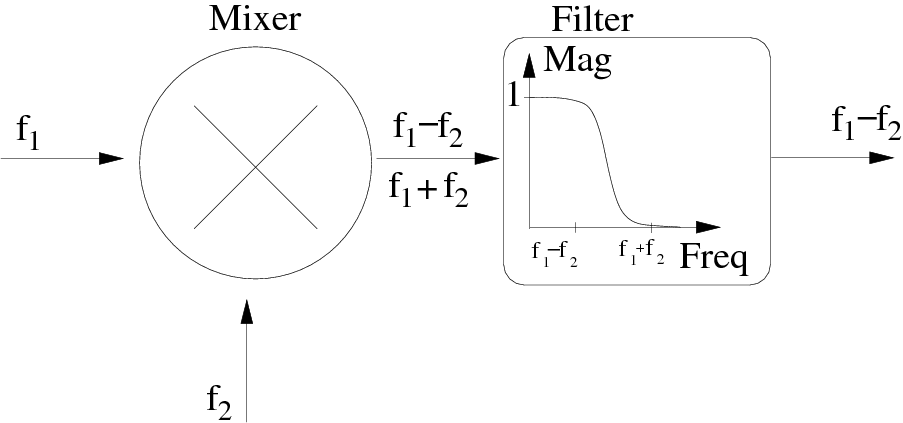
\includegraphics[scale=0.50]{analogue_mixer.png}
%\caption{Test Picture for lof (List of Figures) Display Test Purpose Only
%[The file used is in PDF format.]}

%\label{fig:A.1}

%\end{figure}

%\begin{figure}[ht]
%\centering
%\includegraphics[scale=0.60]{TestPattern1.bmp}
%\caption{CS4270 Test Bench 1 FPGA Design Diagram
%[Picture is for test display purpose only. No meaning.]}

%\label{fig:A.2}

%\end{figure}

% Add this code if you want to get the "Page" word on top of the TOC for the corresponding page. 
%\addtocontents{toc}{\protect\afterpage{~\hfill{Page}\par\medskip}}

\subsection{TEST1}
Test subsection for toc display purpose only.

%\begin{figure}[ht]
%\centering
%\includegraphics[scale=0.90]{TESTOUT3_2bit_2.bmp}
%\caption{Behavioral simulation for TEST1
%[Picture is for test display purpose only. No meaning.]}

%\label{fig:A.3}

%\end{figure}

\subsection{TEST2}
\begin{lstlisting}[language={Verilog},tabsize=12,]
  Begin
     
      If ( shift == 1'b1)
         Begin
         
         sr[(N-1):1] <= sr[(N-2):0];
sr[0] <= sr_in;
end
else
begin
sr[(N-1):1] <= sr[(N-2):0];
sr[0] <= sr[(N-1)];
end
end
\end{lstlisting}

\section{Random Pictures and Test}
Section here is to test toc display purpose only.

\section{Misc Test}
Section here is to test toc display purpose only.

\chapter{SOURCE CODE}

**Some text here**

\section{Misc Test 2}
Section here is to test toc display purpose only.

\section{Misc Test 3}
Section here is to test toc display purpose only.

\section{Resource Usage}
\begin{landscape}
\noindent
Design Summary (This page shows how to use landscape format in Appendix.)\\
\texttt{---------}\\
Design Summary:\\
Number of errors: 0\\
Number of warnings: 0\\
Logic Utilization:\\
Number of Slice Flip Flops: 3,899 out of 33,280 11\%\\
Number of 4 input LUTs: 3,717 out of 33,280 11\%\\
Logic Distribution:\\
Number of occupied Slices: 2,198 out of 16,640 13\%\\
Number of Slices containing only related logic: 2,198 out of 2,198 100\%\\
Number of Slices containing unrelated logic: 0 out of 2,198 0\%\\
*See NOTES below for an explanation of the effects of unrelated logic.\\
Total Number of 4 input LUTs: 3,890 out of 33,280 11\%\\

\end{landscape}


\begin{landscape}
\begin{table}[htbp]


 \label{table:B.1}
 
 \caption{Summary of Equipment Used}
 
\begin{tabular}{|c|c|c|}
\hline
\textbf{NAME} & \textbf{NO}. & \textbf{COMMENT}\\
\hline
Tektronix TDS7704B Scope & 1 & 7GHz, 20GSa/s time-equivallent sampling oscilloscope\\
\hline
Tektronix P7240 Probe & 2 & 4GHz Single Ended Active Probe(High Impedance)\\
\hline
Agilent 81130A Function Generator & 1 & 2 CHs Signal Generator \\
\hline
Xilinx Spartan-3A DSP 1800A Demo Board & 1 & \url{http://goo.gl/Svvpy}\\
\hline

\end{tabular}
\begin{tablenotes} 
\small 
\item
\relax
[By University Requirement, no text should be allowed here in this landscape table/picture page. \textbf{DON'T USE sidewaystable from rotating package, it cannot align landscape title to the left binding side.]} 
\end{tablenotes}
\end{table}
\end{landscape}

